\documentclass[dvipdfmx,fleqn]{beamer}
%\documentclass[dvipdfmx,fleqn,handout]{beamer}
\usepackage{amsmath,amssymb,amsthm}

\mode<presentation>
{
  \usetheme{default}
}

\title{\Large Fictitious Play}
\author{\large 山岸 敦}
\date{\small 2014/6/28}

\usefonttheme{professionalfonts}

\setbeamercovered{transparent=20}

\setbeamertemplate{navigation symbols}{} 
\setbeamertemplate{footline}[frame number] 



\begin{document}

\sffamily
\gtfamily


\begin{frame}
  \titlepage
  \thispagestyle{empty}
\end{frame}

\setcounter{framenumber}{0}




\begin{frame}
\frametitle{構成}
\begin{itemize}\setlength{\parskip}{0.5em}
\item
Fictitious Playとは?
\item
シミュレーション結果の解説
 \begin{itemize}\setlength{\parskip}{0.5em}
 \item
Matching Pennies Game
 \item
 Coordination Game
 \end{itemize}

\item
Pythonコードの解説
\end{itemize}
\end{frame}



\begin{frame}
\frametitle{Fictitious Playの解説}
\begin{itemize}\setlength{\parskip}{0.5em}
\item
Ficititious playでは、相手の前回の行動により、「相手がどの手をどんな確率で出してくるか」についての予想(信念)が変化する状況が想定されます。\pause

\item
さらにどの時点でも、プレイヤーは「その時点での自信の信念に照らして最適」な行動をするとします。このとき、各人の信念の動きはどうなるのでしょうか?\pause
\item
信念の推移を定式化すると、(導出は省略しますが) 

$x_0(t)$ は
\[
x_0(t+1)
= x_0(t) + \frac{1}{t+2} (a_1(t) - x_0(t))
\]
と再帰的に書くことができます。 



\end{itemize}
\end{frame}

\begin{frame}
\frametitle{Matching Pennies Gameの解説}
\begin{itemize}\setlength{\parskip}{0.5em}
\item
Matching Pennies Gameの利得行列は
\[\left( \begin{array}{cc}
(1,-1) & (-1,1) \\
(-1,1) & (1,-1) 
\end{array} \right)\]
です。ナッシュ均衡は両戦略に確率(0.5,0.5)ずつ付与する混合戦略のみであることがわかります。\pause

\item
お互いの信念が(0.5,0.5)に収斂するならば、ナッシュ均衡が実現する、と考えてよいでしょう\pause
\item
本当にそうなるか、シミュレーションした結果を示します。



\end{itemize}
\end{frame}


\begin{frame}
\frametitle{}
\begin{figure}
 \centering
 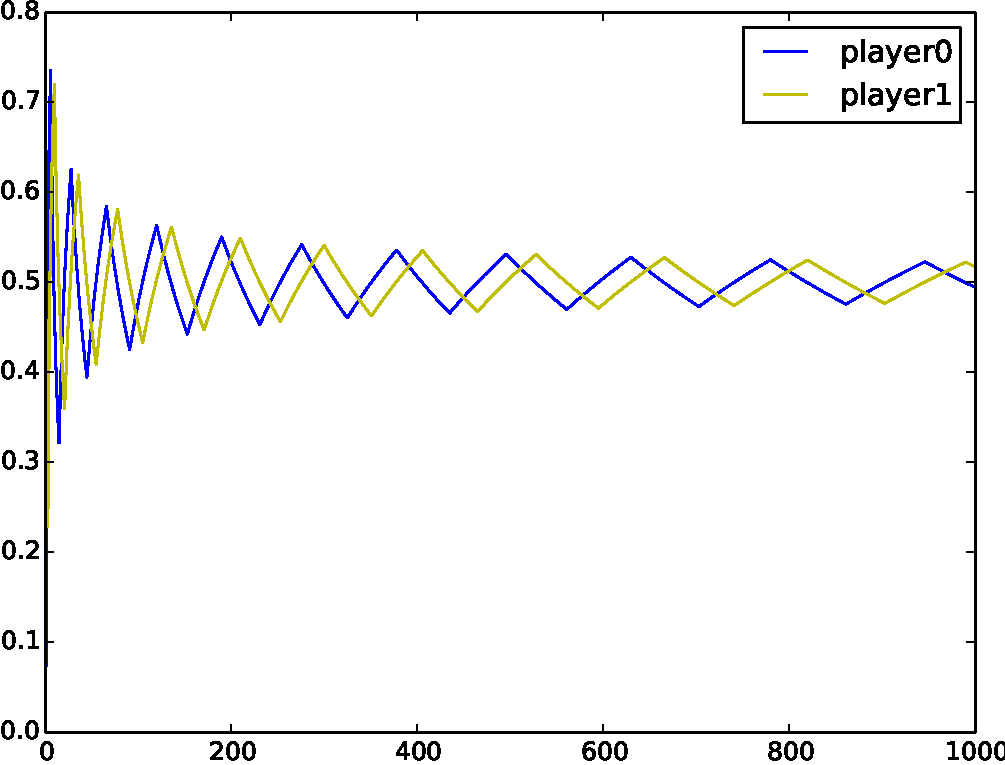
\includegraphics[scale=0.58, bb=-250 -200 250 200]{fictitious_graph1.0.pdf}
 \caption{Matching Pennies Game}
 \label{fig:matchingpennies_plot}
\end{figure}
\end{frame}

\begin{frame}
\frametitle{}
\begin{figure}
 \centering
 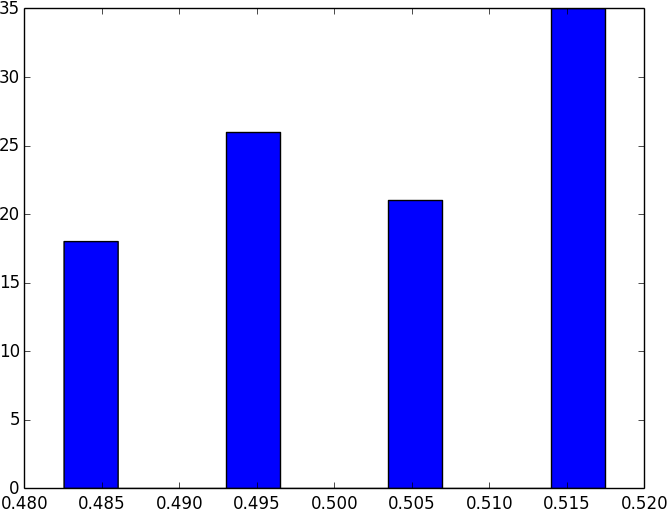
\includegraphics[scale=0.58, bb=-250 -200 250 200]{fictitious_histo1.0.png}
 \caption{Matching Pennies Game}
 \label{fig:matchingpennies_histo}
\end{figure}
\end{frame}

\begin{frame}
\frametitle{Coordination Gameの解説}
\begin{itemize}\setlength{\parskip}{0.5em}
\item
Coordination Gameの利得行列は
\[\left( \begin{array}{cc}
(4,4) & (0,3) \\
(3,0) & (2,2) 
\end{array} \right)\]
です。ナッシュ均衡は純粋戦略の組(0,0)、(1,1)および、2人とも確率(2/3,1/3)ずつ付与する混合戦略の3つです。\pause

\item
先程とちがって、ナッシュ均衡が複数あります。このケースではどのようなプレイがなされるのでしょうか\pause
\item
本当にそうなるか、シミュレーションした結果を示します。



\end{itemize}
\end{frame}

\begin{frame}
\frametitle{}
\begin{figure}
 \centering
 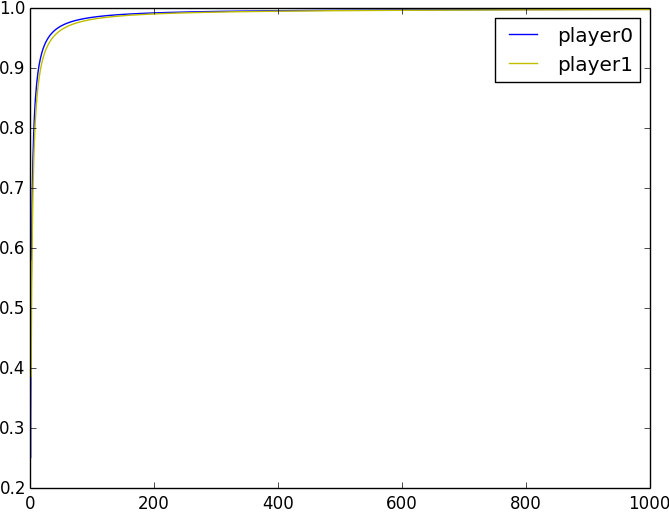
\includegraphics[scale=0.58, bb=-250 -200 250 200]{coordinationgame_graph1.png.png}
 \caption{Coordination Game}
 \label{fig:coordination_plot1}
\end{figure}
\end{frame}


\begin{frame}
\frametitle{}
\begin{figure}
 \centering
 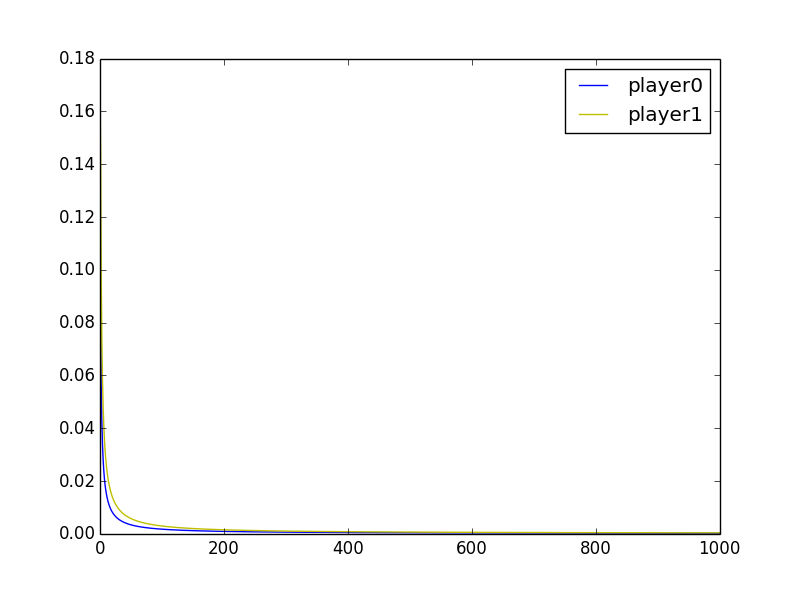
\includegraphics[scale=0.58, bb=100 200 400 300]{coordinationgame_graph2.png}
 \label{fig:coordination_plot2}
\end{figure}
\end{frame}

\begin{frame}
\frametitle{}
\begin{figure}
 \centering
 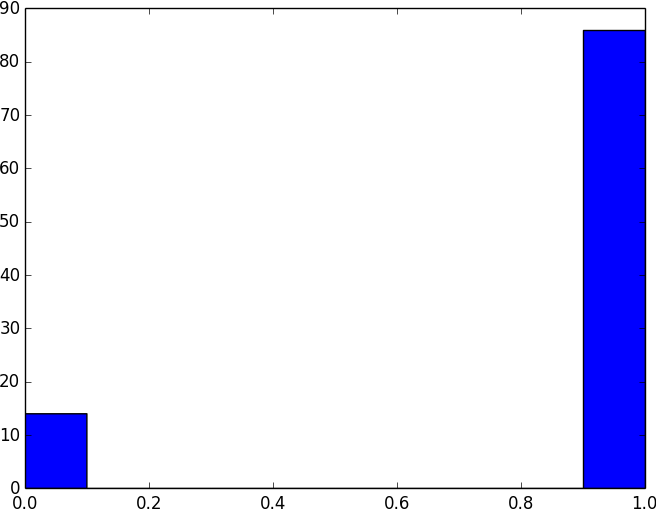
\includegraphics[scale=0.58, bb=-250 -200 250 200]{coordination_histo1.0.png}
 \caption{Coordination Game}
 \label{fig:coordination_histo}
\end{figure}
\end{frame}




\begin{frame}
\frametitle{補足:Coordination Game}
\begin{itemize}\setlength{\parskip}{0.5em}
\item
計算するとわかりますが、各プレイヤーは「相手が2/3より大きいの確率で0をプレイするなら0を、それが2/3より小さければ1を」必ず選択します。このことから、混合戦略均衡で、たまたまお互いに0ないし1を取ればそちらの均衡に移るとわかります。 \pause
\item
「相手が均衡(純)戦略を取る確率が$p$以上の時、自分もその均衡(純)戦略を取るのが最適である」とき、その戦略の組み合わせは$p$-ドミナントと呼ばれます。\pause
\item
計算すると、(0,0)は2/3ドミナント、(1,1)は1/3ドミナントです。1/3のが小さいので、「相手が均衡(純)戦略を取る確率がより低くても最適で在り続ける」という意味で安全な均衡と考えられます。 \pause
\item
ヒストグラムを眺めると、混合戦略に収斂した回数はゼロで、また(0,0)均衡と比して(1,1)均衡がプレイされる頻度が圧倒的に大きいですが、それはこのような理論的背景による、と考えられます。


\end{itemize}
\end{frame}




\begin{frame}[containsverbatim]% verbatim 環境を使えるように
\frametitle{コードの説明とか}
\begin{itemize}\setlength{\parskip}{0.5em}
\item
コードの表示の例
\begin{verbatim}
import numpy
from matplotlib import pyplot

x = numpy.arange(0, 10, 0.1)
y = numpy.cos(x)
pyplot.plot(x,y)
pyplot.show()
\end{verbatim}

\item
\verb|\begin{frame}| から \verb|\end{frame}| までを
コピー\&ペーストしてスライドを増やしていく.
\end{itemize}
\end{frame}



\begin{frame}
\frametitle{まとめ}
\begin{itemize}\setlength{\parskip}{0.5em}
\item
まとめ

\item
よくわかっていない点とか

\item
今後の課題とか
\end{itemize}
\end{frame}




\end{document}